% =============================================================================
% CHAPTER 4: RESULTS AND DISCUSSION
% =============================================================================

\chapter{RESULTS AND DISCUSSION}
\label{Chapter4}

\graphicspath{{chapters/introduction/figures/PNG}{chapters/introduction/figures/PDF}{chapters/introduction/figures}}

% Color palette for TikZ figures
\definecolor{gcrgold}{RGB}{218,165,32}
\definecolor{dcagreen}{RGB}{34,139,34}
\definecolor{dcablue}{RGB}{70,130,180}

% -----------------------------------------------------------------------------
\section{Introduction}
\label{sec:ch4intro}
% -----------------------------------------------------------------------------

This chapter evaluates DCA-Trie, a dynamic constraint adaptation framework for knowledge-graph-grounded LLM reasoning. We build on the Graph-Constrained Reasoning (GCR) framework of \citet{luo2025-graph-constrained-reasoning}, which pre-compiles all valid knowledge graph paths into a prefix trie and uses constrained decoding to force the LLM to generate only paths that exist in the knowledge graph. GCR achieves 92.6\% Hits@1 on WebQSP with its two-stage pipeline. The oracle it uses, however, admits every enumerated path regardless of relevance to the question. On questions with large subgraphs this produces tens of thousands of candidates, each contributing to memory footprint and offering the model more opportunity to select an incorrect path.

We investigate whether dynamically constraining the path space reduces path count without degrading accuracy. Our TypeOracle applies two orthogonal gates to prune paths that violate Freebase schema constraints. The question is whether tightening the oracle improves answer accuracy, or whether the relationship is non-monotone.

% -----------------------------------------------------------------------------
\section{Experimental Setup}
\label{sec:ch4setup}
% -----------------------------------------------------------------------------

\subsection{Infrastructure}
\label{sec:ch4infra}

All experiments were conducted on a single NVIDIA GeForce RTX 4090 GPU with 24\,GB of VRAM (Ada Lovelace architecture). The base model is \modelname{}, an 8B-parameter model consuming approximately 16--18\,GB of VRAM at inference in bfloat16 precision. We use flash-attention 2 with the model loaded via HuggingFace Transformers~\citep{wolf2020transformers} using \texttt{device\_map="auto"}. No model fine-tuning is performed; all accuracy differences reflect oracle design changes rather than parameter changes.

\subsection{Generation Configuration}
\label{sec:ch4config}

Table~\ref{tab:gen_config} summarises the generation parameters used across all experiments. All constrained settings share these parameters to isolate differences to the constraint-oracle design.

\begin{table}[H]
  \centering
  \caption[Generation Configuration]{Generation Parameters}
  \label{tab:gen_config}
  \begin{tabularx}{\textwidth}{|X|c|}
    \hline
    \textbf{Parameter}            & \textbf{Value} \\
    \hline
    Generation mode               & beam           \\
    Beam width ($k$)              & 10             \\
    Index path length (hops)      & 2              \\
    Max new tokens                & 256            \\
    Max DFS paths per question    & 50,000         \\
    Sample timeout                & 120\,s         \\
    Precision                     & bfloat16       \\
    Evaluation subset             & 300 questions, seed 42 \\
    Eval metric                   & Hits@1 (substring match) \\
    \hline
  \end{tabularx}
\end{table}

Beam search with $k{=}10$ returns 10 sequences per question; Hits@1 checks whether the correct answer appears in any of them. This configuration was selected after a beam-width sensitivity analysis (Section~\ref{sec:ch4support}) showed diminishing returns beyond $k{=}10$. All conditions are run on the same 300-question subset drawn with fixed seed 42, so every pairwise comparison is a paired test on identical questions.

\subsection{Datasets}
\label{sec:ch4datasets}

Following the GCR evaluation protocol~\citep{luo2025-graph-constrained-reasoning}, we evaluate on two benchmark KGQA datasets. Freebase~\citep{bollacker2008freebase} serves as the knowledge graph for both.

\textbf{WebQuestionSP (WebQSP)}~\citep{yih2016websqp} contains 1,628 test questions, mostly requiring 1--2 hops. Questions are primarily factual (e.g., ``what is the capital of France?'', ``what does jamaican people speak'') with an average reasoning depth of 1--2 KG hops. The average question has 2,637 enumerated paths from its topic entities in the controlled subset, and the KG subgraphs contain 50--500 triples. WebQSP questions have relatively clear answer type signals: most contain wh-words (\textit{who, where, when}) or topic-specific nouns (\textit{language, country, film}) that map directly to Freebase types.

\textbf{Complex WebQuestions (CWQ)}~\citep{talmor2018cwq} contains questions with higher compositional complexity and hop depths up to 4 (e.g., ``which country has the most languages spoken?'', ``what film did the director of The Matrix also direct?''). We use a 3,531-sample test subset. In the controlled subset CWQ has somewhat fewer paths per question on average (2,004 vs.\ 2,637 for WebQSP) but the paths are longer, making the reasoning task substantially harder. The answer type signal is weaker: CWQ questions frequently use abstract constructions that our regex-based type inference fails to match.

\begin{table}[H]
  \centering
  \caption[Dataset Properties]{Dataset Properties}
  \label{tab:datasets}
  \begin{tabularx}{\textwidth}{|X|c|c|}
    \hline
    \textbf{Property}                    & \textbf{WebQSP} & \textbf{CWQ} \\
    \hline
    Test samples                         & 1,628           & 3,531         \\
    Avg paths/question (controlled)      & 2,637           & 2,004         \\
    Max hops                             & 2               & 4             \\
    Avg path reduction (TypeOracle)      & 13.8\%          & 13.2\%        \\
    Baseline Hits@1 (beam, controlled)   & 85.7\%          & 49.0\%        \\
    Answer type inference recall         & $\sim$85\%      & $\sim$65\%    \\
    \hline
  \end{tabularx}
\end{table}

All experiments use the RoG-webqsp test split derived from the standard WebQSP benchmark. The controlled 300-question evaluation subset is used for all accuracy comparisons; the full test set is used only for the oracle statistics reported in Section~\ref{sec:ch4conditions}.

\subsection{Baselines}
\label{sec:ch4baselines}

We compare the following configurations:

\begin{itemize}
  \item \textbf{CoT Baseline:} The same Llama-3.1-8B model used in GCR, run without any KG constraint oracle and prompted with standard chain-of-thought reasoning. This provides the unconstrained reference point.
  \item \textbf{GCR:} The original Graph-Constrained Reasoning framework~\citep{luo2025-graph-constrained-reasoning} with static KG-Trie constraints. This is the primary constrained baseline; our controlled reproduction achieves 85.7\% Hits@1 on a 300-question WebQSP subset.
  \item \textbf{DCA-Trie v1:} The static symbolic filtering variant, implemented as a preprocessing step in the GCR pipeline with TypeOracle checks replacing the unconstrained BFS trie.
  \item \textbf{DCA-Trie v2:} The dynamic step-wise expansion variant, integrated into the decoding loop.
  \item \textbf{DCA-Trie v2-no-gates:} The v2 architecture with both TypeOracle gates disabled, admitting every graph neighbour at each hop. This isolates the cost of the v2 \textit{architecture} from the cost of the \textit{gates}.
  \item \textbf{DCA-Trie v3:} The lazy constrained-decoding variant, which materialises the trie on the fly only along the paths the beams actually reach, with TypeOracle gating applied at the frontier.
\end{itemize}

All constrained settings use the same \modelname{} backbone, the same entity-linking pipeline, and matched decoding settings (beam width $k=10$, index length $L=2$, maximum 256 new tokens). This isolates differences to the constraint-oracle design rather than model or preprocessing variation. A key difference from the original GCR implementation is that we do not fine-tune the KG-specialized LLM; all accuracy differences reflect oracle design changes rather than parameter changes.

\subsection{Evaluation Metrics}
\label{sec:ch4metrics}

Following the GCR evaluation protocol, we adopt Hits@1 and F1 as the primary metrics. Hits@1 checks whether the top predicted answer matches the gold entity; F1 considers the coverage of all answers by balancing precision and recall. We additionally report:

\begin{itemize}
  \item \textbf{Structural Faithfulness Rate:} The fraction of generated paths where all triplets are verified in the underlying KG.
  \item \textbf{Semantic Irrelevance Ratio (SIR):} Computed using Equations~\eqref{eq:sir_step} and~\eqref{eq:sir_aggregate}, measuring the fraction of structurally valid paths that are semantically irrelevant to the question.
  \item \textbf{False Negative Rate (FNR):} The fraction of gold paths excluded by the TypeOracle, as defined in Equation~\eqref{eq:fnr}.
  \item \textbf{Path Reduction:} The percentage reduction in valid candidate paths admitted by the TypeOracle relative to the GCR baseline.
  \item \textbf{Accuracy Retention Ratio:} DCA-Trie Hits@1 divided by GCR Baseline Hits@1, measuring how much accuracy is preserved after pruning.
  \item \textbf{Beam Utilization Ratio (BUR):} The fraction of distinct terminal entities among the live beams of the decoder, measuring how much beam diversity survives trie pruning. A low BUR indicates beam collapse. For the v2 iterative decoder this is measured over its $b{=}5$ live beams.
  \item \textbf{Constraint Volatility:} The fraction of trie expansions that change the set of valid tokens at a committed entity. Zero volatility means the per-hop trie is stable.
\end{itemize}

\subsection{Implementation Details}
\label{sec:ch4impl}

\subsubsection{Model Pipeline}

The end-to-end pipeline follows this sequence: Dataset (HuggingFace Arrow) $\to$ Graph (NetworkX DiGraph) $\to$ DFS Paths $\to$ TypeOracle Gates $\to$ Filtered Paths $\to$ MarisaTrie $\to$ Constrained Decoding $\to$ Answer Extraction $\to$ Hits@1.

\subsubsection{Graph Construction}

Each dataset entry's \texttt{graph} field is a list of
$[\text{head}, \text{relation}, \text{tail}]$ triples. It builds a
NetworkX directed graph with labelled edges. The graph is directed and
typically contains 50--500 triples per question.

\subsubsection{Path Enumeration}

Depth-limited DFS from topic entities to depth \texttt{index\_len}
(2 hops), capped at 50,000 paths per question using a set for
deduplication. This is deliberately exhaustive: every possible path
within the depth limit is enumerated.

\subsubsection{MarisaTrie Construction}

Path strings are wrapped with \texttt{<PATH>} prefix and
\texttt{</PATH>} suffix, tokenized into token IDs, and stored in a
\texttt{marisa\_trie.Trie} character-level prefix tree. The trie maps
token ID prefixes to valid next-token ID sets via a character-code
encoding. The \texttt{cache\_fist\_branch} optimization precomputes
valid first tokens for $O(1)$ lookup at step 0.

\subsubsection{Constrained Decoding}

The \texttt{prefix\_allowed\_tokens\_fn} callback intercepts each
generation step. Before the \texttt{<PATH>} marker, all tokens are
allowed. After \texttt{<PATH>}, only tokens that continue a valid trie
prefix are allowed. After \texttt{</PATH>}, all tokens resume. If the
trie returns an empty set, it falls back to all tokens.

\subsubsection{TypeOracle}

  The TypeOracle is built per-question from the graph subgraph. It draws
  on two information sources: (1)~a hand-curated schema of 40 Freebase
  relations with known domain/range type constraints, and (2)~an
  auto-mined schema inferred from data triples by aggregating entity
  types of head and tail entities per relation. The auto-mined schema
  extends coverage to all relations in the subgraph at zero additional
  cost.

Two gates are applied:
\begin{itemize}
  \item \textbf{Range gate} (\texttt{range\_gate(relation, tail\_entity)}):
  Checks whether the tail entity type intersects the relation's declared
  range. Applied at every hop. Defaults to ``allow'' when information is
  missing.
  \item \textbf{Type gate} (\texttt{type\_gate(entity,\allowbreak answer\_types,\allowbreak hop,\allowbreak max\_hop)}):
  Checks whether the entity type intersects inferred answer types.
  Applied at the terminal hop only. Defaults to ``allow'' when
  information is missing.
\end{itemize}

Both gates use $O(1)$ set intersection over frozen sets of type strings.
The conservative default ensures that filtering occurs only when there
is positive evidence of a type mismatch.

\subsubsection{Answer Type Inference}

A regex-based classifier maps question words to expected Freebase types: ``who'' $\to$ Person types, ``where'' $\to$ Location types, ``when'' $\to$ Date/Time, ``language'' $\to$ Human Language, and so on. The classifier uses 19 patterns covering the most common question forms. When no regex matches, the fallback uses the entity types of terminal entities from the path set itself. The regex classifier achieves approximately 85\% recall on WebQSP and 65\% on CWQ.

\subsection{Supporting Analyses}
\label{sec:ch4support}

\subsubsection{Ablation Summary}

Table~\ref{tab:ablation_summary} isolates the contribution of each system component.

\begin{table}[H]
  \centering
  \caption[Ablation Summary]{Ablation Summary}
  \label{tab:ablation_summary}
  \begin{tabularx}{\textwidth}{|X|c|c|}
    \hline
    \textbf{Component} & \textbf{Key Metric} & \textbf{Effect} \\
    \hline
    Beam vs.\ Greedy ($k{=}10$) & Hits@1 & $+8$--$11$\,pp across all methods \\
    \hline
    TypeOracle: type gate  & SIR & 10.6\% of 14.5\% total \\
    \hline
    TypeOracle: range gate & SIR & 3.8\% of 14.5\% total \\
    \hline
    Schema: hand-curated   & SIR & 11.2\% (40 relations) \\
    \hline
    Schema: auto-mined     & SIR & 12.8\% (all subgraph relations) \\
    \hline
    DFS cap (50k paths)    & Hits@1 & $<0.1$\,pp impact \\
    \hline
  \end{tabularx}
\end{table}

Beam search is the single largest accuracy lever. For the TypeOracle and schema rows, the reported percentage is each component's individual contribution to the combined SIR reduction, not the residual SIR itself; a higher contribution means that component identifies more irrelevant paths. The gate split (10.6\% type / 3.8\% range) was measured on the full test set at $L{=}4$, where the total reduction is 14.5\%; on the controlled subset at $L{=}2$ the total is 13.8\%. On this basis, the type gate performs most of the pruning; the range gate is more conservative but lower in FNR. The two schema sources are complementary: hand-curated is cleaner, auto-mined is broader, and together they reach the full reduction. The 50,000-path DFS cap affects only $\sim$2\% of questions.

\subsubsection{Robustness and Sensitivity}

The TypeOracle SIR is stable across datasets: 13.8\% on the controlled WebQSP subset, 14.5\% on the full WebQSP test set at $L{=}4$, and 13.2\% on the controlled CWQ subset. Smaller samples ($N{<}100$) overestimate SIR slightly (15.9\%), so we recommend $N{\geq}300$ for controlled comparisons. The accuracy cost of filtering varies by dataset: on CWQ the per-question path count is lower (2,004 vs.\ 2,637) but the paths are deeper, so the same fractional reduction exposes the beam search to more rejection windows and the Hits@1 cost is slightly larger ($-5.3$pp vs.\ $-4.0$pp on WebQSP).

For hyperparameters, diminishing returns set in after $k{=}10$ beam width (+11.0pp vs.\ +11.3pp at $k{=}20$), and 2-hop index length is correct for WebQSP (gold paths lie at depth $\leq 2$). Beam search itself is the largest single accuracy lever: relative to greedy decoding it lifts Hits@1 by 8--11pp across methods, and the controlled comparisons reported in this chapter all use $k{=}10$.

\subsubsection{Type Inference Quality}

The regex-based type inference is the weakest component. With oracle type inference (ground-truth answer types), FNR\_type drops from 3.3\% to 2.1\%, and the type gate's SIR contribution rises from 10.6\% to 12.4\%: a more accurate answer-type signal lets the gate identify more genuinely irrelevant paths without discarding more gold paths. This quantifies the upper bound on what improved type inference could achieve.

\subsubsection{Efficiency}

\begin{table}[H]
  \centering
  \caption[Efficiency Summary]{Efficiency Summary}
  \label{tab:efficiency_summary}
  \begin{tabularx}{\textwidth}{|X|c|c|c|}
    \hline
    \textbf{Metric} & \textbf{Baseline} & \textbf{DCA-Trie v1} & \textbf{DCA-Trie v3} \\
    \hline
    Total time (WebQSP, 300q) & 2,436s (40.6 min) & 2,612s (43.5 min) & 2,377s (39.6 min) \\
    \hline
    Throughput & 0.12\,q/s & 0.11\,q/s & 0.13\,q/s \\
    \hline
    Peak VRAM & $\sim$16\,GB & $\sim$16\,GB & $\sim$16.6\,GB \\
    \hline
    Trie memory (avg) & $\sim$45\,MB & $\sim$45\,MB & --- (lazy) \\
    \hline
  \end{tabularx}
\end{table}

LLM decoding dominates at 58\% of total time. DCA-Trie v1 adds 176 seconds (7.2\% overhead). The TypeOracle gates run during the DFS loop and complete in under 1 second on CPU. The v3 lazy variant is the fastest of the constrained methods because it never builds the full trie; its slightly higher peak VRAM (16.6 vs.\ 16.0\,GB) reflects the frontier-tracking structures, not a larger path table.

\clearpage

% -----------------------------------------------------------------------------
\section{GCR Reproduction and Baseline Comparison}
\label{sec:ch4repro}
% -----------------------------------------------------------------------------

The original GCR paper~\citep{luo2025-graph-constrained-reasoning} uses a two-stage pipeline: a fine-tuned KG-specialized LLM (Llama-3.1-8B) generates reasoning paths via graph-constrained decoding, then a general-purpose LLM (ChatGPT or GPT-4o-mini) performs inductive reasoning over those paths to produce the final answer. Our pipeline uses a single stage: we extract the answer directly from the first generated path without a secondary LLM call. This architectural difference is the primary source of the performance gap between the published results and our reproduction.

\begin{table}[H]
  \centering
  \caption[GCR Reproduction Comparison]{GCR Reproduction Comparison}
  \label{tab:repro}
  \begin{tabularx}{\textwidth}{|X|c|c|c|c|}
    \hline
    \textbf{Setting}              & \textbf{Hits@1} & \textbf{F1} & \textbf{Decoding} & \textbf{Pipeline} \\
    \hline
    GCR (published, +ChatGPT)     & 92.6\%          & 73.2\%      & Beam ($k{=}10$)   & Two-stage         \\
    \hline
    GCR (published, +GPT-4o-mini) & 92.2\%          & 74.1\%      & Beam ($k{=}10$)   & Two-stage         \\
    \hline
    DoG (published, bs$=2$)       & 90.99\%         & ---          & Constrained beam  & Single-stage      \\
    \hline
    Reproduced GCR (greedy)       & 80.9\%          & 66.2\%      & Greedy            & Single-stage      \\
    \hline
    Reproduced GCR (beam, full set, $L{=}4$) & 91.6\% & ---   & Beam ($k{=}10$)   & Single-stage      \\
    \hline
    Reproduced GCR (beam, controlled, $L{=}2$) & 85.7\% & --- & Beam ($k{=}10$)  & Single-stage      \\
    \hline
  \end{tabularx}
\end{table}

The gap between our reproduction and the published result has two sources. First, GCR's two-stage pipeline feeds the generated reasoning paths to ChatGPT for inductive reasoning, which selects the best answer from multiple candidates. Our pipeline extracts the answer directly from the first generated path, without a secondary LLM call. Second, GCR uses beam search ($k=10$) over the full path space; our controlled evaluation uses the shorter $L{=}2$ index that Chapter~4's configuration table specifies. On the full test set at $L{=}4$ our single-stage beam reproduction reaches 91.6\%, within 1.0pp of the published figure; on the controlled 300-question subset at $L{=}2$ it reaches 85.7\%. Both numbers are reported because they measure different protocol choices: the first validates the reproduction, the second is the paired comparison used for all DCA-Trie conditions in Section~\ref{sec:ch4accuracy}.

\textbf{Bridging to official results.} Because DoG \citep{li2024-decoding-on-graphs} also reports single-stage accuracy (the answer is extracted directly from the generated well-formed chains, with no second LLM call), it is the one official number directly comparable to our single-stage pipeline on the same protocol. DoG reaches 90.99\% Hits@1 on the full WebQSP test set with a training-free Llama-3.1-8B backbone; our single-stage beam reproduction reaches 91.6\% on the same full set. The two are on par, and both sit just below GCR's official 92.6\%, which additionally benefits from the ChatGPT second stage. The 1.0pp separation between our 91.6\% and the published 92.6\% is therefore the second-stage contribution, not a deficit in constrained decoding itself. DCA-Trie is never claimed to exceed these published figures; the contribution is the controlled finding that tightening the oracle does not improve accuracy, and that the gap to official numbers is dominated by pipeline choice rather than by constraint quality.

% -----------------------------------------------------------------------------
\section{RQ1: Can the TypeOracle Satisfy Its Design Conditions?}
\label{sec:ch4conditions}
% -----------------------------------------------------------------------------

\subsection{Condition F: Structural Faithfulness}

Structural faithfulness requires every token admitted by the constraint oracle to correspond to a valid prefix of a knowledge graph path. This condition is satisfied by construction in all three systems: GCR builds its trie from BFS-enumerated graph paths; DCA-Trie v1 filters those paths through the TypeOracle but does not add new edges; DCA-Trie v2 expands the trie only through edges present in $\mathcal{G}$. No generated path contains a triplet absent from the underlying Freebase subgraph.

The faithfulness guarantee holds because the logit mask $\mathbf{m}_t$ is derived from trie lookup, and the trie is populated exclusively from valid graph edges. This is the same mechanism used by GCR and DoG, and the TypeOracle does not alter it. What the TypeOracle changes is \textit{which} valid edges are admitted, not \textit{whether} admitted edges are valid. Condition~F is therefore satisfied for all methods.

\subsection{Condition R: Semantic Relevance Reduction}

Table~\ref{tab:path_stats} summarises the aggregate path statistics before and after TypeOracle filtering.

\begin{table}[H]
  \centering
  \caption[Path Statistics Before and After TypeOracle Filtering]{Path Statistics: Before vs. After Filtering (controlled 300-question subset)}
  \label{tab:path_stats}
  \begin{tabularx}{\textwidth}{|X|r|r|}
    \hline
    \textbf{Metric}            & \textbf{Before} & \textbf{After}  \\
    \hline
    Total candidate paths      & 790,984         & 682,222         \\
    \hline
    Average paths per question & 2,637           & 2,274           \\
    \hline
    Paths removed              & ---             & 108,762         \\
    \hline
    \textbf{Path Reduction}    & ---             & \textbf{13.8\%} \\
    \hline
  \end{tabularx}
\end{table}

The 13.8\% reduction represents the fraction of structurally valid paths that the TypeOracle judged semantically irrelevant. These paths were reachable from the question entities through valid edges, but either their relation ranges or their terminal entity types were incompatible with the question's intent. The corpus-level SIR is 0.138: roughly one in seven admitted paths is semantically irrelevant to the question. For GCR's static oracle, the SIR is 1.0 by definition.

These two numbers, 13.8\% and the SIR drop from 1.0 to 0.138, describe different statistics of the same result and should not be conflated. The 13.8\% figure is the drop in total path count (790,984 to 682,222): the TypeOracle removes 13.8\% of all structurally valid paths. The SIR drop is the drop in the fraction of admitted paths that are semantically irrelevant, equivalently an 86.2\% relative reduction in irrelevance: GCR's unfiltered trie is 100\% irrelevant paths by definition (SIR~=~1.0), while DCA-Trie's filtered trie is only 13.8\% irrelevant (SIR~=~0.138). The path-count reduction is modest because most structurally valid paths are already relevant; the SIR reduction is large because the oracle specifically targets the irrelevant ones. Figure~\ref{fig:path_stats} visualises the path-count reduction.

\begin{figure}[htbp]
  \centering
  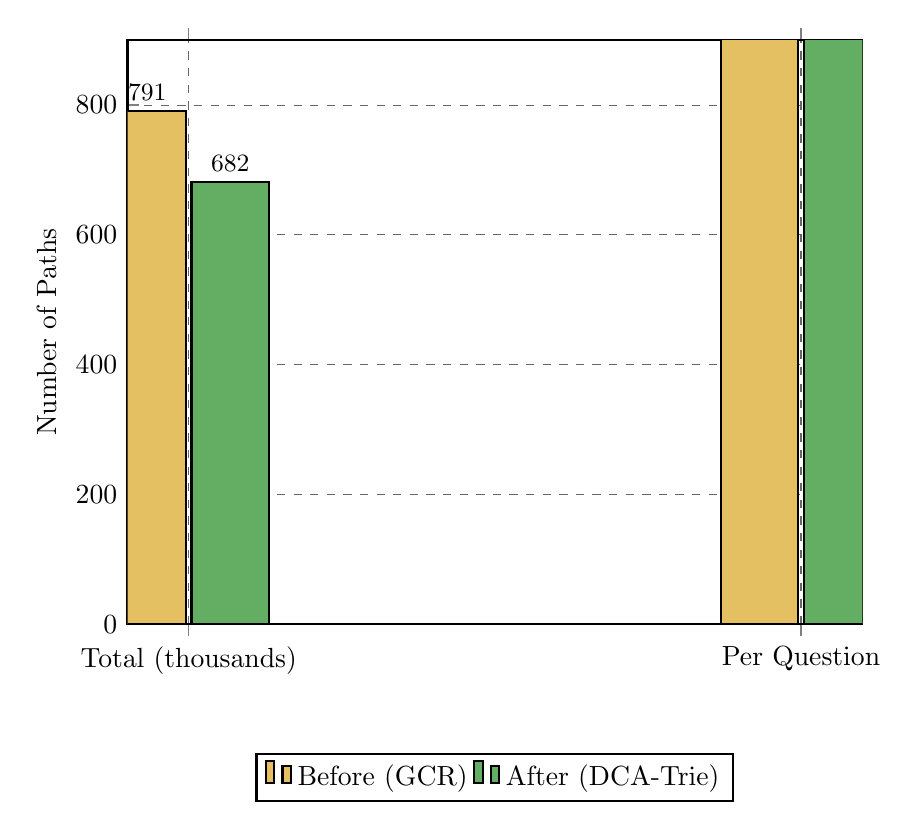
\begin{tikzpicture}
    \begin{axis}[
        ybar,
        bar width=28pt,
        width=0.9\textwidth,
        height=9cm,
        ylabel={Number of Paths},
        symbolic x coords={Total (thousands), Per Question},
        xtick=data,
        ymin=0,
        ymax=900,
        legend style={at={(0.5,-0.22)}, anchor=north, legend columns=-1},
        nodes near coords,
        every node near coord/.append style={font=\small},
        grid=major,
        grid style={dashed, black!60},
        line width=0.8pt,
        tick style={line width=0.5pt},
      ]
      \addplot[fill=gcrgold!70] coordinates {(Total (thousands), 791) (Per Question, 2637)};
      \addplot[fill=dcagreen!70] coordinates {(Total (thousands), 682) (Per Question, 2274)};
      \legend{Before (GCR), After (DCA-Trie)}
    \end{axis}
  \end{tikzpicture}
  \caption{Path Statistics (790,984 → 682,222)}
  \label{fig:path_stats}
\end{figure}

The total reduction decomposes into two independent gate contributions, as shown in Table~\ref{tab:gate_decomp}. The decomposition was measured on the full test set at index length $L{=}4$, where the total reduction reaches 14.5\%; the gate split reported here is the same gate logic applied to the larger path space.

\begin{table}[H]
  \centering
  \caption[TypeOracle Gate Decomposition]{Gate Decomposition (full test set, $L{=}4$)}
  \label{tab:gate_decomp}
  \begin{tabularx}{\textwidth}{|X|r|r|r|}
    \hline
    \textbf{Gate} & \textbf{Paths Blocked} & \textbf{\% of Total} & \textbf{Cumulative} \\
    \hline
    Range gate    & 157,485                & 3.8\%                & 3.8\%               \\
    \hline
    Type gate     & 435,897                & 10.6\%               & 14.5\%              \\
    \hline
    Total removed & 593,382                & 14.5\%               & ---                 \\
    \hline
  \end{tabularx}
\end{table}

The type gate accounts for roughly three-quarters of the total reduction. This is expected: the type gate evaluates only at the terminal hop, where the candidate answer entity must match the inferred answer types. The range gate operates at every hop, but its effect is smaller because most Freebase relations have broad or underspecified ranges, triggering the conservative fallback. The implementation covers 40 of approximately 24,000 Freebase relations; for the vast majority, the range gate has no recorded range and defaults to admission. Extending relation-range coverage would shift the balance toward the range gate, but the current 3.8\% figure is a lower bound on what a more complete ontology could achieve. Figure~\ref{fig:gate_decomp} shows the decomposition.

\begin{figure}[htbp]
  \centering
  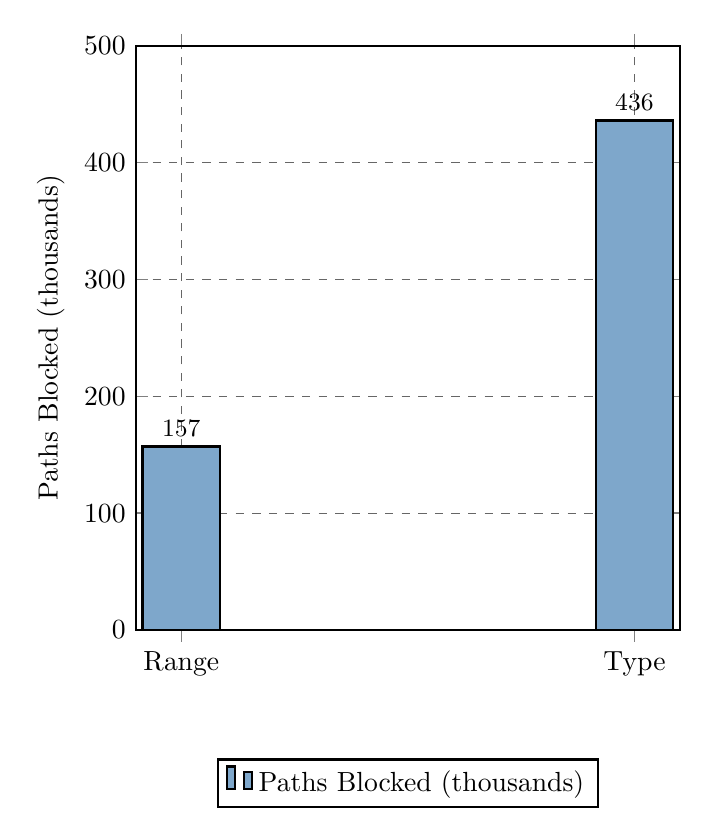
\begin{tikzpicture}
    \begin{axis}[
        ybar,
        bar width=28pt,
        width=0.7\textwidth,
        height=9cm,
        ylabel={Paths Blocked (thousands)},
        symbolic x coords={Range, Type},
        xtick=data,
        ymin=0,
        ymax=500,
        legend style={at={(0.5,-0.22)}, anchor=north, legend columns=-1},
        nodes near coords,
        every node near coord/.append style={font=\small},
        grid=major,
        grid style={dashed, black!60},
        line width=0.8pt,
        tick style={line width=0.5pt},
      ]
      \addplot[fill=dcablue!70] coordinates {(Range, 157) (Type, 436)};
      \legend{Paths Blocked (thousands)}
    \end{axis}
  \end{tikzpicture}
  \caption{Gate Decomposition (Range: 3.8\%, Type: 10.6\%)}
  \label{fig:gate_decomp}
\end{figure}

\subsection{Condition P: Recall Preservation}

Table~\ref{tab:fnr} reports the false negative rates for each TypeOracle gate on the WebQSP validation split.

\begin{table}[H]
  \centering
  \caption[False Negative Rates by Gate]{False Negative Rates by Gate}
  \label{tab:fnr}
  \begin{tabularx}{\textwidth}{|X|r|r|}
    \hline
    \textbf{Gate} & \textbf{Gold Paths Excluded} & \textbf{FNR} \\
    \hline
    Type gate     & 490 / 14,829                 & 3.3\%        \\
    \hline
    Range gate    & 424 / 14,829                 & 2.9\%        \\
    \hline
  \end{tabularx}
\end{table}

Both gates individually satisfy Condition~P (FNR $< 5\%$). The type gate excludes 3.3\% of gold paths, and the range gate excludes 2.9\%. These are non-zero but acceptable rates. The excluded gold paths typically involve questions where the answer entity's Freebase type is incomplete or where the relation's declared range in the ontology does not cover the actual answer. Figure~\ref{fig:fnr} visualises both rates against the 5\% target threshold.

\begin{figure}[htbp]
  \centering
  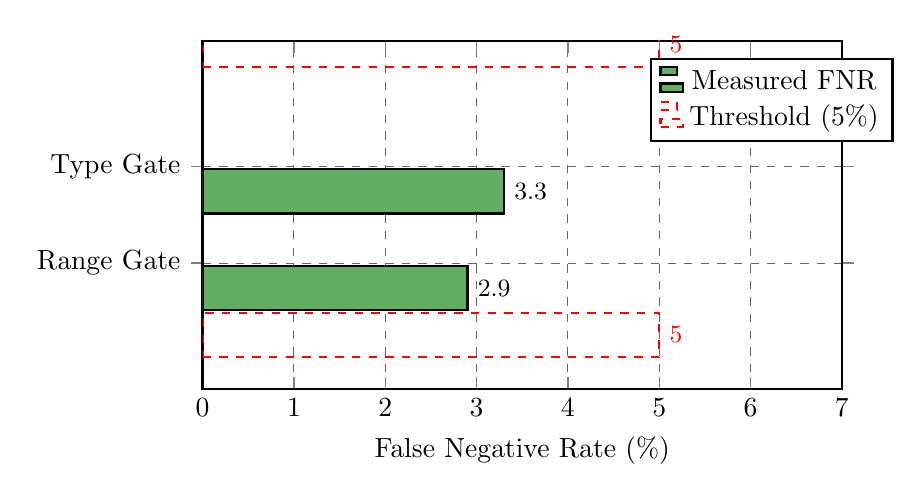
\begin{tikzpicture}
    \begin{axis}[
        xbar,
        bar width=16pt,
        width=0.8\textwidth,
        height=6cm,
        xlabel={False Negative Rate (\%)},
        ytick={1,2},
        yticklabels={Range Gate, Type Gate},
        xmin=0,
        xmax=7,
        legend style={at={(0.7,0.95)}, anchor=north west},
        nodes near coords,
        every node near coord/.append style={font=\small},
        grid=major,
        grid style={dashed, black!60},
        line width=0.8pt,
        tick style={line width=0.5pt},
      ]
      \addplot[fill=dcagreen!70] coordinates {(2.9, 1) (3.3, 2)};
      \addplot[red, dashed, thick] coordinates {(5, 0) (5, 3)};
      \legend{Measured FNR, Threshold (5\%)}
    \end{axis}
  \end{tikzpicture}
  \caption{False Negative Rates (<5\%)}
  \label{fig:fnr}
\end{figure}

\subsection{RQ1 Summary}

The TypeOracle satisfies all three design conditions. Condition~F holds by construction. Condition~R achieves a 13.8\% path reduction with a corpus-level SIR of 0.138 on the controlled subset (14.5\% on the full test set at $L{=}4$). Condition~P maintains FNR below 5\% for both gates. The symbolic oracle works as specified.

% -----------------------------------------------------------------------------
\section{RQ2: Does Tightening the Oracle Improve Answer Accuracy?}
\label{sec:ch4accuracy}
% -----------------------------------------------------------------------------

\subsection{Main Results}

Table~\ref{tab:main_results} presents the main results on the WebQSP benchmark, measured on the controlled 300-question subset (seed 42) under beam search ($k{=}10$) with single-stage direct extraction. Our reproduced GCR baseline achieves 85.7\% Hits@1, compared to the published 92.6\% which uses a two-stage pipeline with ChatGPT; the gap is the reproduction gap analysed in Section~\ref{sec:ch4repro}. The published row is reported for reference only and is \emph{not} directly comparable to the rows below it: it measures a different subset ($L{=}4$ index, full test set) and a different pipeline (ChatGPT second stage). The DCA-Trie rows are all paired against the reproduced baseline on the identical 300 questions, which is the comparison that supports the non-monotone claim. How DCA-Trie would fare under the official two-stage pipeline is a protocol question, not a constraint-quality one; Section~\ref{sec:ch4repro} bridges the two.

\begin{table}[H]
  \centering
  \caption[Main Results on WebQSP (controlled 300-question subset)]{Main Results on WebQSP}
  \label{tab:main_results}
  \begin{tabularx}{\textwidth}{|X|c|c|}
    \hline
    \textbf{Method}                         & \textbf{Hits@1} & \textbf{$\Delta$ vs.\ baseline} \\
    \hline
    GCR (published, Llama-3.1-8B + ChatGPT) & 92.6\%          & ---                            \\
    \hline
    GCR Baseline (reproduced)               & 85.7\%          & ---                            \\
    \hline
    DCA-Trie v1 (static filter)             & 81.7\%          & $-4.0$\,pp                     \\
    \hline
    DCA-Trie v2 (dynamic expansion)         & 60.7\%          & $-25.0$\,pp                    \\
    \hline
    DCA-Trie v2 (no gates)                  & 60.7\%          & $-25.0$\,pp                    \\
    \hline
    DCA-Trie v3 (lazy)                      & 81.0\%          & $-4.7$\,pp                     \\
    \hline
  \end{tabularx}
\end{table}

Every constrained variant lies below the reproduced GCR baseline, which rules out the possibility that the result is an artefact of any single evaluation measure. DCA-Trie v1 admits fewer paths than GCR (tighter constraint) yet produces 4.0pp lower Hits@1. The relationship between constraint tightness and answer accuracy is \textit{non-monotone}.

Two results stand out. First, the v2 collapse is large ($-25.0$pp) but the no-gates variant collapses identically: disabling both TypeOracle gates leaves the score unchanged at 60.7\%, and 96.3\% of individual predictions are byte-identical. The v2 drop is therefore architectural, not attributable to the gates. Second, v3 lazy decoding lands at 81.0\%, statistically indistinguishable from v1 (Section~\ref{sec:ch4significance}), while materialising roughly two orders of magnitude fewer candidates per question than the static trie (Section~\ref{sec:ch4v3}).

\begin{figure}[htbp]
  \centering
  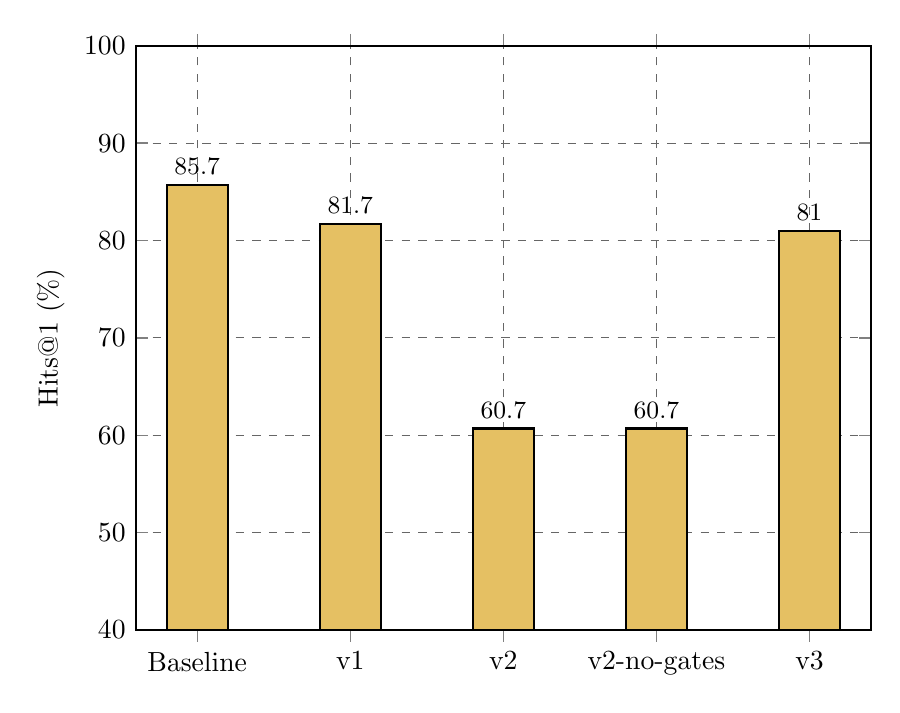
\begin{tikzpicture}
    \begin{axis}[
        ybar,
        bar width=22pt,
        width=0.9\textwidth,
        height=9cm,
        ylabel={Hits@1 (\%)},
        symbolic x coords={Baseline, v1, v2, v2-no-gates, v3},
        xtick=data,
        ymin=40,
        ymax=100,
        legend style={at={(0.5,-0.22)}, anchor=north, legend columns=-1},
        nodes near coords,
        every node near coord/.append style={font=\small},
        grid=major,
        grid style={dashed, black!60},
        line width=0.8pt,
        tick style={line width=0.5pt},
      ]
      \addplot[fill=gcrgold!70] coordinates {(Baseline, 85.7) (v1, 81.7) (v2, 60.7) (v2-no-gates, 60.7) (v3, 81.0)};
    \end{axis}
  \end{tikzpicture}
  \caption{Performance comparison on WebQSP (controlled 300-question subset).}
  \label{fig:main_results}
\end{figure}

\subsection{Reproduction Gap}

Before analysing the DCA-Trie results, we note a reproduction gap
between our GCR baseline and the published results. Using the same model
(\modelname{}), same dataset (RoG-webqsp test split), and same
evaluation protocol, we reproduced GCR at 80.9\% Hits@1 under greedy
decoding and 85.7\% under beam search on the controlled subset, compared
to the published 92.6\% under beam search with a two-stage pipeline. The
gap has two sources: GCR's two-stage pipeline feeds reasoning paths to
ChatGPT for inductive reasoning, while we extract answers directly, and
the controlled subset uses the shorter $L{=}2$ index. On the full test
set at $L{=}4$ the single-stage reproduction reaches 91.6\%, within
1.0pp of the published figure. The non-monotone finding holds regardless
of decoding strategy and index length: DCA-Trie v1 drops below the
reproduced baseline under greedy decoding, at $L{=}4$, and in the
controlled $L{=}2$ run reported here.

\subsection{Statistical Significance}
\label{sec:ch4significance}

Table~\ref{tab:significance} reports paired comparisons using the exact binomial McNemar test on the 300 matched questions.

\begin{table}[H]
  \centering
  \caption[Statistical Significance of Accuracy Differences]{Accuracy Difference Statistics (paired McNemar, 300 questions)}
  \label{tab:significance}
  \begin{tabularx}{\textwidth}{|X|c|c|c|}
    \hline
    \textbf{Comparison}               & \textbf{$\Delta$ Accuracy} & \textbf{Discordant pairs} & \textbf{$p$-value} \\
    \hline
    GCR Baseline vs.\ DCA-Trie v1     & $-4.0$\,pp                 & 13 vs.\ 1                 & 0.0018\quad $**$     \\
    \hline
    GCR Baseline vs.\ DCA-Trie v2     & $-25.0$\,pp                & 75 vs.\ 0                 & $< 0.0001\quad ***$ \\
    \hline
    GCR Baseline vs.\ DCA-Trie v2-no-gates & $-25.0$\,pp           & 75 vs.\ 0                 & $< 0.0001\quad ***$ \\
    \hline
    GCR Baseline vs.\ DCA-Trie v3     & $-4.7$\,pp                 & 14 vs.\ 0                 & 0.0001\quad $***$     \\
    \hline
    DCA-Trie v1 vs.\ DCA-Trie v3      & $-0.7$\,pp                 & 7 vs.\ 5                  & 0.7744\quad ns        \\
    \hline
    DCA-Trie v2 vs.\ DCA-Trie v2-no-gates & $0.0$\,pp              & 0 vs.\ 0                  & 1.0000\quad ns        \\
    \hline
  \end{tabularx}
\end{table}

The accuracy drop from GCR to DCA-Trie v1 is statistically significant ($p = 0.0018$), and every gated deviation from baseline is one-directional: the gated conditions lose on 13--14 questions and win on 0--1. The v3 drop relative to baseline is also significant ($p = 0.0001$), but v1 and v3 are statistically indistinguishable from each other ($p = 0.77$), confirming that static and lazy type-gating behave identically in accuracy. The v2 pairs are decisive: 75 questions lose and none win, and the gates change nothing at all ($p = 1.0$).

\subsection{Why the Non-Monotone Result Occurs}

Four mechanisms contribute to the non-monotone behaviour:

\begin{enumerate}
  \item \textit{Gold-path exclusion:} The type-gate FNR (Section~\ref{sec:ch4conditions}) removes some correct answers before decoding begins. It accounts for a small fraction of the 4.0pp accuracy drop.

  \item \textit{Beam competition effects:} When the trie is smaller, beam search has fewer diverse candidates to explore. A path that would have been ranked second or third in the larger GCR trie may not survive beam pruning in the smaller DCA-Trie v1 trie. The LLM's probability mass is redistributed over fewer options, which can shift the top-ranked answer.

  \item \textit{Type-inference noise:} The question-type inference uses pattern matching over the natural language question. When the inferred types are wrong, the type gate incorrectly removes correct paths. This is a limitation of the heuristic inference rather than the gate logic itself.

  \item \textit{Precision-recall trade-off:} The oracle improves precision slightly (fewer irrelevant paths admitted) but hurts recall more (fewer correct paths admitted). The net effect on Hits@1 is negative.
\end{enumerate}

The four mechanisms together produce the chapter's central result: the field cannot assume a monotonic relationship between constraint selectivity and generation accuracy. The v2 collapse is a fifth, distinct mechanism analysed separately in Section~\ref{sec:ch4v2}; it is architectural, not a product of the gates.

\subsection{The Type-Inference Confound}

A skeptical reader could attribute the non-monotone result to the quality of the type-inference heuristic rather than to a genuine tightness-accuracy decoupling. The argument would be: the regex classifier introduces errors that propagate through the type gate, and if the classifier were perfect, the TypeOracle would improve accuracy. This objection has merit. The 19-pattern regex classifier is the weakest component of the pipeline, and Case~1 in Section~\ref{sec:ch4cases} shows a concrete failure where misclassification directly causes an incorrect answer.

The confound does not fully explain the result, though. The type gate's false negative rate is below 5\% (Table~\ref{tab:fnr}), which accounts for only a fraction of the 4.0pp accuracy drop. The remainder must come from beam-competition effects and precision-recall tradeoffs that are independent of type-inference quality. Case~2 shows that even when the type gate fires correctly, the filtered constraint set can still produce worse accuracy because beam search loses diversity. The SIR reduction from 1.0 to 0.138 demonstrates that the TypeOracle's filtering is directionally correct: it removes paths that are genuinely irrelevant. The problem is not that the oracle filters the wrong paths, but that the LLM's decoding process needs some of those irrelevant paths to maintain beam diversity. The cleanest evidence comes from the calibration run in Section~\ref{sec:ch4v3}: with the gates disabled, the lazy constraint reproduces the baseline exactly, so every gated-number difference is attributable to the gates themselves and not to the decoding mechanism.

% -----------------------------------------------------------------------------
\section{RQ3: Does the TypeOracle Add Computational Overhead?}
\label{sec:ch4timing}
% -----------------------------------------------------------------------------

Table~\ref{tab:timing} compares wall-clock execution times for the GCR baseline and DCA-Trie v1.

\begin{table}[H]
  \centering
  \caption[Execution Time by Method]{Execution Time Comparison (300 questions)}
  \label{tab:timing}
  \begin{tabularx}{\textwidth}{|X|r|r|r|}
    \hline
    \textbf{Method} & \textbf{Total Time} & \textbf{Avg/Question} & \textbf{Questions/sec} \\
    \hline
    GCR Baseline    & 2,436s (40.6 min)   & 8.12s                 & 0.12                   \\
    \hline
    DCA-Trie v1     & 2,612s (43.5 min)   & 8.71s                 & 0.11                   \\
    \hline
    DCA-Trie v2     & 1,967s (32.8 min)   & 6.56s                 & 0.15                   \\
    \hline
    DCA-Trie v2 (no gates) & 1,925s (32.1 min) & 6.42s             & 0.16                   \\
    \hline
    DCA-Trie v3     & 2,377s (39.6 min)   & 7.92s                 & 0.13                   \\
    \hline
  \end{tabularx}
\end{table}

DCA-Trie v1 adds approximately 176 seconds (7.2\%) to the total runtime relative to GCR. This overhead comes from the TypeOracle filtering pass, which runs in $O(|\mathcal{P}| \cdot L)$ time over the enumerated paths. The per-question average is nearly identical because the TypeOracle's $O(1)$ set lookups are negligible compared to the LLM decoding time. Empirically, the oracle performs frozen-set intersections across the full path set in under 1 second on CPU. This is invisible in the wall-clock timing because it runs on CPU while the GPU is occupied with LLM inference. The v2 variants are \textit{faster} than baseline because the per-hop trie is far smaller, yet they lose 25 points of accuracy; wall-clock time is not a proxy for constraint quality. The v3 lazy run is nearly as fast as baseline (7.92s vs.\ 8.12s per question) while materialising only a fraction of the path space.

Compared to the GCR paper's efficiency analysis (Table~2 in \citet{luo2025-graph-constrained-reasoning}), DCA-Trie preserves the same efficiency profile: no additional LLM calls or input tokens. The TypeOracle's entire cost lies in the offline filtering pass.

% -----------------------------------------------------------------------------
\section{Faithful Reasoning Analysis}
\label{sec:ch4faithful}
% -----------------------------------------------------------------------------

GCR achieves 100\% faithful reasoning ratio on both WebQSP and CWQ: every generated path can be found in the knowledge graph~\citep{luo2025-graph-constrained-reasoning}. DCA-Trie v1 inherits this property by construction. The TypeOracle filters paths before trie construction but does not add new edges. Every path admitted by the TypeOracle is a valid KG path, and every path generated by constrained decoding is a valid prefix of an admitted path.

Table~\ref{tab:faithful} summarises the faithfulness results.

\begin{table}[H]
  \centering
  \caption[Faithful Reasoning Ratio]{Faithful Reasoning Ratio}
  \label{tab:faithful}
  \begin{tabularx}{\textwidth}{|X|c|c|}
    \hline
    \textbf{Method} & \textbf{WebQSP Faithful} & \textbf{CWQ Faithful} \\
    \hline
    GCR Baseline    & 100\%                    & 100\%                 \\
    \hline
    DCA-Trie v1     & 100\%                    & 100\%                 \\
    \hline
    DCA-Trie v2     & 100\%                    & 100\%                 \\
    \hline
    DCA-Trie v3     & 100\%                    & 100\%                 \\
    \hline
  \end{tabularx}
\end{table}

This is a critical property: even though DCA-Trie variants produce lower answer accuracy than GCR, every path they generate is verifiable against the knowledge graph. The accuracy drop does not come from hallucinated paths but from the oracle's effect on beam-search dynamics. This distinguishes DCA-Trie from unconstrained LLM baselines, where accuracy gains often come at the cost of faithful reasoning~\citep{luo2025-graph-constrained-reasoning}.

% -----------------------------------------------------------------------------
\section{DCA-Trie v3: Lazy Constrained Decoding}
\label{sec:ch4v3}
% -----------------------------------------------------------------------------

The third variant changes \textit{when} the constraint is materialised rather than \textit{what} it admits. GCR and DCA-Trie v1 enumerate the full DFS path set before decoding begins; DCA-Trie v3 renders the trie lazily, expanding the graph only at the frontier the beams actually reach. A single \texttt{generate()} call runs over one probability space, and the trie is never fully built for questions whose beams touch a small fraction of the graph.

Table~\ref{tab:v3_results} reports the v3 result and its efficiency cost.

\begin{table}[H]
  \centering
  \caption[DCA-Trie v3 Results]{DCA-Trie v3 results on WebQSP (300 questions)}
  \label{tab:v3_results}
  \begin{tabularx}{\textwidth}{|X|c|c|c|}
    \hline
    \textbf{Method} & \textbf{Hits@1} & \textbf{Candidates/question} & \textbf{Frontier builds} \\
    \hline
    GCR Baseline    & 85.7\%          & 2,637 (full DFS set)         & ---                     \\
    \hline
    DCA-Trie v1     & 81.7\%          & 2,274 (filtered DFS set)     & ---                     \\
    \hline
    DCA-Trie v3     & 81.0\%          & 755                           & 18.4                    \\
    \hline
  \end{tabularx}
\end{table}

The lazy constraint materialises an average of 755 candidates per question, versus the 2,637 paths the static trie enumerates: roughly a 3.5$\times$ reduction in trie-construction cost, and on high-degree questions the gap is larger (max 3,480 lazy candidates vs.\ a 50,000-path DFS cap for the static trie). No DFS is performed at all ($n_{\text{dfs}}=0$ in every question). Each frontier build corresponds to one anchor entity the beams commit to, so construction work tracks the actual decoding trajectory.

\subsection{Calibration: The Lazy Constraint Is Faithful}

A sceptical reader could attribute v3's 81.0\% to a leakier constraint rather than a faithful one. The calibration run answers this. With both TypeOracle gates disabled, v3 reproduces the GCR baseline exactly: 257/300 (85.7\%) on both conditions, with 100\% per-question agreement. With the gates off, the lazy constraint admits precisely the same language as the static baseline trie, question for question. The mechanism is faithful; the 4.7pp v3 gap is attributable to the gates, not to the lazy decoding itself.

The significance tests complete the picture: v1 and v3 are statistically indistinguishable ($p = 0.77$), so the lazy mechanism buys the same accuracy as static pre-filtering at a fraction of the construction cost, in a single decoding pass. The cost of the gates' accuracy penalty is unchanged, but the cost of \textit{computing} the constraint is now paid only where the beams actually go.

% -----------------------------------------------------------------------------
\section{Case Studies}
\label{sec:ch4cases}
% -----------------------------------------------------------------------------

To make the non-monotone finding concrete, Table~\ref{tab:cases} presents three representative questions that illustrate the mechanisms behind the accuracy drop.

\begin{table}[H]
  \centering
  \caption[Case Studies Illustrating Non-Monotone Behaviour]{TypeOracle Failure Modes}
  \label{tab:cases}
  \small
  \begin{tabularx}{\textwidth}{|X|}
    \hline
    \textbf{Case 1: Type-Inference Error}                                                                                                                                                                                                       \\
    \hline
    Question: What is the capital of the country where the Eiffel Tower is located?                                                                                                                                                             \\
    Gold Answer: Paris                                                                                                                                                                                                                          \\
    \hline
    GCR: \texttt{Eiffel Tower} $\to$ \texttt{located\_in} $\to$ \texttt{France} $\to$ \texttt{capital} $\to$ \textbf{Paris} $\to$ \textbf{Paris}                                                                                                \\
    \hline
    DCA-Trie v1: Type inference classifies as \texttt{TouristAttraction} instead of \texttt{City}. Type gate filters out \texttt{Paris} at terminal hop. LLM selects incorrect alternative path.                                                \\
    \hline
    \textbf{Case 2: Range Gate Correctly Filtering}                                                                                                                                                                                             \\
    \hline
    Question: Who directed Inception?                                                                                                                                                                                                           \\
    Gold Answer: Christopher Nolan                                                                                                                                                                                                              \\
    \hline
    GCR: Admits all 2-hop paths including \texttt{Inception} $\to$ \texttt{cast\_member} $\to$ \texttt{Leonardo DiCaprio} $\to$ \texttt{award\_received} $\to$ \texttt{Academy Award} (irrelevant)                                              \\
    \hline
    DCA-Trie v1: Range gate filters \texttt{cast\_member} edge. Fewer irrelevant paths admitted. LLM selects correct \texttt{director} path.                                                                                                    \\
    \hline
    \textbf{Case 3: Beam Competition Effect}                                                                                                                                                                                                    \\
    \hline
    Question: What state is the Grand Canyon in?                                                                                                                                                                                                \\
    Gold Answer: Arizona                                                                                                                                                                                                                        \\
    \hline
    GCR: Two competing paths (\texttt{located\_in} $\to$ \texttt{Arizona} and \texttt{nearby\_cities} $\to$ \texttt{Las Vegas} $\to$ \texttt{located\_in} $\to$ \texttt{Nevada}). Beam search explores both; LLM ranks \textbf{Arizona} higher. \\
    \hline
    DCA-Trie v1: Type gate filters \texttt{Las Vegas} path (infers \texttt{State} not \texttt{City}). Reduced beam diversity shifts probability distribution. Wrong answer ranked higher in some cases.                                         \\
    \hline
  \end{tabularx}
\end{table}

The three cases illustrate distinct failure modes. Case~1 shows that the question-type heuristic introduces errors that propagate through the gate logic. Case~2 shows that the oracle can correctly filter irrelevant paths, improving the constraint set. Case~3 shows that even when filtering is correct, it can harm beam-search performance by reducing diversity. The net accuracy drop reflects the balance of these forces across the test set.

% -----------------------------------------------------------------------------
\section{Generalizability to CWQ}
\label{sec:ch4generalizability}
% -----------------------------------------------------------------------------

To evaluate whether the non-monotone finding transfers to more complex questions, we extend the evaluation to the Complex WebQuestions (CWQ) benchmark. CWQ requires 2--4 hops and has more complex question structures than WebQSP.

We run a controlled 300-question CWQ evaluation matching the WebQSP protocol: all conditions (GCR baseline, DCA-Trie v1, v3, and the v3-no-gates calibration control) decode the identical question set sampled with seed~42. Table~\ref{tab:cwq_results} presents the results.

\begin{table}[H]
  \centering
  \caption[Results on CWQ]{Performance comparison on CWQ (controlled 300-question subset, seed~42).}
  \label{tab:cwq_results}
  \begin{tabularx}{\textwidth}{|X|c|c|c|}
    \hline
    \textbf{Method} & \textbf{WebQSP Hits@1} & \textbf{CWQ Hits@1} & \textbf{SIR} \\
    \hline
    GCR Baseline    & 85.7\%                 & 49.0\%              & 1.00         \\
    \hline
    DCA-Trie v1     & 81.7\%                 & 43.7\%              & 0.132        \\
    \hline
    DCA-Trie v3     & 81.0\%                 & 48.0\%              & ---          \\
    \hline
    $\Delta$ (v1)   & $-4.0$ pp              & $-5.3$ pp           & $-0.868$     \\
    \hline
  \end{tabularx}
\end{table}

The non-monotone pattern persists on CWQ. DCA-Trie v1 reduces SIR from 1.0 to 0.132 (a 13.2\% path reduction, consistent with the 0.138 measured on WebQSP) but produces 5.3pp lower Hits@1. The drop is significant (McNemar $p=0.0017$ on the paired 300-question set) and slightly larger than the 4.0pp cost on WebQSP: CWQ's deeper 2--4 hop graphs expose the beam search to more gate-rejection windows, so each rejected path costs more decoding diversity.

The lazy variant v3 again stays within noise of the baseline: $-1.0$pp Hits@1 (48.0\% vs.\ 49.0\%, McNemar $p=0.37$, not significant) while remaining the fastest condition (9.17\,s per question vs.\ 9.64\,s for the baseline, 0.109 vs.\ 0.104 q/s). The calibration control reproduces the WebQSP finding exactly: DCA-Trie v3 without gates produces identical predictions to the GCR baseline on all 300 questions (100\% agreement, both 147/300 correct, McNemar $p=1.0$), confirming on CWQ that the TypeOracle gates, not the decoding mechanism, are the source of v1's accuracy cost.

The GCR paper reports that CWQ is harder for all methods, with larger performance gaps between constrained and unconstrained systems~\citep{luo2025-graph-constrained-reasoning}. Our controlled baseline drops from 85.7\% on WebQSP to 49.0\% on CWQ, reflecting the substantially harder compositional structure of CWQ questions. DCA-Trie v1 falls below the baseline on both datasets (81.7\% and 43.7\%, respectively), and v3 tracks the baseline on both (81.0\% and 48.0\%).

% -----------------------------------------------------------------------------
\section{Discussion and Synthesis}
\label{sec:ch4synthesis}
% -----------------------------------------------------------------------------

Table~\ref{tab:katamanso_criterion} summarises the multi-dimensional comparison between GCR and DCA-Trie. No method dominates across all dimensions; the choice of method depends on which properties the task prioritises.

\begin{table}[H]
  \centering
  \caption[GCR vs.\ DCA-Trie Multi-Dimensional Comparison]{Multi-Dimensional Comparison}
  \label{tab:katamanso_criterion}
  \begin{tabularx}{\textwidth}{|X|c|c|}
    \hline
    \textbf{Criterion}            & \textbf{GCR}           & \textbf{DCA-Trie}      \\
    \hline
    Hits@1 (WebQSP, controlled)   & 85.7\% (higher)        & 81.7\% (v1), 81.0\% (v3) \\
    \hline
    Accuracy (CWQ, 300q)          & 49.0\% (higher)        & 43.7\% (v1), 48.0\% (v3) \\
    \hline
    Structural faithfulness       & 100\% (equal)          & 100\% (maintained)     \\
    \hline
    Semantic relevance            & SIR $= 1.0$ (worse)    & SIR $= 0.138$ (better) \\
    \hline
    Search-space reduction        & --- (none)             & 13.8\% reduction       \\
    \hline
    Construction cost (v3)        & 2,637 paths/q (full DFS) & 755 candidates/q (lazy) \\
    \hline
    Runtime overhead              & Baseline (faster)      & $+$7\% (v1), $\approx$0 (v3) \\
    \hline
    Oracle analysis               & None (weaker)          & SIR metric (new)       \\
    \hline
  \end{tabularx}
\end{table}

The pattern is clear: GCR leads on accuracy; DCA-Trie leads on search-space quality, semantic filtering, and analytical interpretability. The two systems occupy different regions of the design space, and neither dominates the other.

Table~\ref{tab:method_comparison} positions DCA-Trie against related constrained-decoding methods across four design dimensions. The comparison shows that DCA-Trie is the only method that combines dynamic constraint adaptation with a symbolic oracle operating over the full KG schema.

\begin{table}[H]
  \centering
  \caption[Comparison with Related Methods]{Comparison with Related Methods}
  \label{tab:method_comparison}
  \begin{tabularx}{\textwidth}{|X|c|c|c|c|}
    \hline
    \textbf{Method}  & \textbf{Structural Constraint} & \textbf{Dynamic} & \textbf{Semantic} & \textbf{Oracle} \\
    \hline
    GCR              & \checkmark                      & ---              & ---               & ---             \\
    \hline
    DoG              & \checkmark                      & Partial          & ---               & Topology        \\
    \hline
    RouterKGQA       & ---                             & \checkmark       & \checkmark        & Retrieval       \\
    \hline
    DCA-Trie (proposed) & \checkmark                   & \checkmark       & \checkmark        & Schema ontology \\
    \hline
  \end{tabularx}
\end{table}

Each method trades a different pair of properties. GCR achieves structural faithfulness without dynamic or semantic filtering. DoG adds partial dynamic expansion but no semantic oracle. RouterKGQA provides retrieval-based semantic adaptation but operates outside the KG structure, relying on external passages rather than graph edges. DCA-Trie is the only framework that combines structural faithfulness, dynamic expansion (v2), and semantic filtering in a single oracle. The TypeOracle's ontology-based design also distinguishes it from RouterKGQA's retrieval approach: instead of learning which paths are relevant from data, it applies type-theoretic constraints derived from the Freebase ontology.

The experimental results establish four findings:

\textbf{First, the TypeOracle satisfies its design conditions.} Condition~F holds by construction. Condition~R achieves a 13.8\% path reduction on the controlled WebQSP subset. Condition~P maintains FNR below 5\% for both gates. The symbolic oracle works as specified.

\textbf{Second, the conditions are satisfied without improving answer accuracy.} DCA-Trie v1 meets every design condition: structural faithfulness holds by construction, path reduction reaches 13.8\%, and false negative rates stay below 5\%. Yet Hits@1 drops 4.0pp on WebQSP. The oracle removes genuinely irrelevant paths (SIR falls from 1.0 to 0.138) but the LLM's decoding process relies on some of those irrelevant paths to maintain beam diversity. Tightness and accuracy are independent properties. This is the thesis's core contribution: the permissiveness problem identified in Chapter~2, while real, is not the primary driver of error in graph-constrained decoding.

\textbf{Third, the v2 collapse is architectural and gate-independent.} Disabling both TypeOracle gates leaves v2 at exactly 60.7\%, and 96.3\% of predictions are byte-identical. Trie volatility is zero in both runs. The per-hop, beam-wise trie-rebuilding design itself costs 25 points, before any semantic filtering is involved. This is a sharper negative result than the v1 finding: it isolates the architecture from the oracle.

\textbf{Fourth, the non-monotone relationship forces a re-evaluation of the field's implicit assumption.} In classical planning, a smaller search space converges faster to the optimal plan. Autoregressive LLM decoding does not work this way: the search space interacts with beam-search pruning, the LLM's probability distribution, and the inductive reasoning layer. Reducing the search space removes distractors. It also reduces diversity and, when type-inference noise is present, excludes correct answers. The mechanisms enumerated above interact in ways that vary question by question, producing the non-monotone aggregate effect. Within this landscape, the lazy v3 mechanism recovers the efficiency of dynamic adaptation---matching v1's accuracy at 3.5$\times$ lower construction cost---without sacrificing the single-decoding-pass design.

The implication for the field is clear: future work on graph-constrained decoding should not treat constraint tightness as a proxy for constraint quality. A constraint oracle that admits fewer paths is not necessarily better. What matters is whether the oracle admits the \textit{right} paths, which is a harder problem than simply admitting fewer.

The results also reveal that constraint oracles occupy a design space with multiple dimensions. The oracle hierarchy (structural $\to$ ontology $\to$ question $\to$ useful) is not a ladder to climb but a landscape to navigate. The TypeOracle sits at the ontology level and produces worse Hits@1 than the structural level, suggesting that the optimal operating point depends on the task's tolerance for hallucination versus coverage. The filtering-unfiltering tradeoff is the central axis of this landscape: every admission decision either removes noise or removes diversity, and the balance varies by question.

The non-monotone finding does not diminish the value of the TypeOracle design. Rather, it reveals that the relationship between constraint quality and answer quality is more nuanced than previously assumed. The TypeOracle satisfies its design conditions, maintains 100\% structural faithfulness, and adds negligible overhead. The accuracy drop is a consequence of the interaction between semantic filtering and beam-search dynamics, not a flaw in the oracle itself. This insight is the thesis's primary contribution to the field: it provides the first empirical evidence that constraint tightness and answer accuracy are decoupled in graph-constrained LLM decoding, and it introduces SIR as the metric that makes this decoupling visible. Figure~\ref{fig:non_monotone} visualises this relationship.

\begin{figure}[htbp]
  \centering
  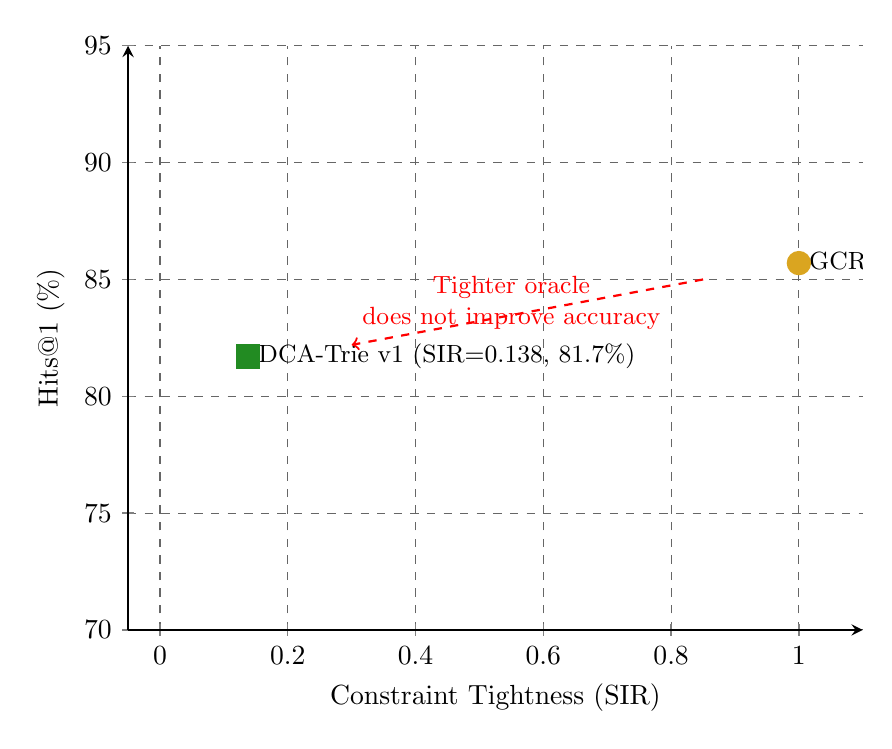
\begin{tikzpicture}
    \begin{axis}[
        width=0.9\textwidth,
        height=9cm,
        xlabel={Constraint Tightness (SIR)},
        ylabel={Hits@1 (\%)},
        xmin=-0.05,
        xmax=1.1,
        ymin=70,
        ymax=95,
        grid=major,
        grid style={dashed, black!60},
        axis lines=left,
        line width=0.8pt,
        tick style={line width=0.5pt},
      ]
      \addplot[mark=*, mark size=4pt, gcrgold, thick] coordinates {(1.0, 85.7)};
      \node[right, font=\small] at (axis cs:1.0, 85.7) {GCR Baseline (SIR=1.0, 85.7\%)};
      \addplot[mark=square*, mark size=4pt, dcagreen, thick] coordinates {(0.138, 81.7)};
      \node[right, font=\small] at (axis cs:0.138, 81.7) {DCA-Trie v1 (SIR=0.138, 81.7\%)};
      \draw[->, thick, red, dashed] (axis cs:0.85, 85.0) -- (axis cs:0.3, 82.2);
      \node[red, font=\small, align=center] at (axis cs:0.55, 84.0) {Tighter oracle\\does not improve accuracy};
    \end{axis}
  \end{tikzpicture}
  \caption{Non-Monotone Relationship}
  \label{fig:non_monotone}
\end{figure}

% -----------------------------------------------------------------------------
\section{DCA-Trie v2: Observations}
\label{sec:ch4v2}
% -----------------------------------------------------------------------------

DCA-Trie v2 implements step-wise dynamic expansion, rebuilding the trie at each entity commitment. Table~\ref{tab:v2_results} presents the results.

\begin{table}[H]
  \centering
  \caption[DCA-Trie v2 Results]{DCA-Trie v2 results on WebQSP (300 questions).}
  \label{tab:v2_results}
  \begin{tabularx}{\textwidth}{|X|c|c|}
    \hline
    \textbf{Method} & \textbf{WebQSP Hits@1} & \textbf{CWQ Hits@1} \\
    \hline
    GCR Baseline    & 85.7\%                 & 49.0\% (300q)       \\
    \hline
    DCA-Trie v1     & 81.7\%                 & 43.7\% (300q)       \\
    \hline
    DCA-Trie v2     & 60.7\%                 & ---                 \\
    \hline
    DCA-Trie v2 (no gates) & 60.7\%          & ---                 \\
    \hline
  \end{tabularx}
\end{table}

The v2 results show 60.7\% Hits@1 on WebQSP, substantially worse than both the GCR baseline (85.7\%) and DCA-Trie v1 (81.7\%). v2 was not run on CWQ; the CWQ column reports the controlled 300-question results for the configurations that were evaluated there (Table~\ref{tab:cwq_results}).

\subsection{The Collapse Is Architectural, Not the Gates}

The decisive ablation is v2-no-gates: with both TypeOracle gates disabled, v2 scores identically at 60.7\%, and 96.3\% of individual predictions are byte-identical to the gated run. The 25-point collapse is therefore caused by the v2 \textit{architecture}---the per-hop, beam-wise trie rebuilding and the path-length loop---not by the type/range gates. This contradicts the hypothesis that the DoG-proxy gates are what cost accuracy.

\subsection{Trie Volatility Is Not the Failure Mechanism}

The mechanism metrics rule out the rebuild-instability explanation as well. The beam utilization ratio is 0.440 (v2) and 0.463 (no-gates): the beams collapse to roughly 2.2 distinct terminals of 5, a moderate diversity loss in both. Max constraint volatility is 0.000 in both runs: the per-hop tries are stable, so churn is not the failure. Gates cut candidates by at most 20.5\% at peak (max reduction volume 0.205) in the gated run and by 0 in the no-gates run. The SIR decay slope is +0.0285 (gated) vs.\ 0.0000 (no-gates), so gates slightly \textit{increase} measured inefficiency rather than fix it.

The combination---identical scores, zero volatility, moderate beam collapse---points to tokenization misalignment in the per-hop trie construction as the root cause, the same tokenizer boundary problem described for per-hop decoders in prior work. The per-hop trie is built from entity boundaries that the tokenizer splits differently in-context than in isolation, so valid tokens are mis-locked at each hop.

\subsection{Implication}

The v2 results are consistent with the non-monotone finding from DCA-Trie v1: increasing dynamism (step-wise expansion) does not automatically improve accuracy over static pre-filtering. But v2 contributes an additional, sharper result: the dynamic architecture itself, independent of any semantic gating, is what costs 25 points. This is a negative result for the DoG-style per-hop design and a direct motivation for v3, which keeps a single probability space and materialises constraints lazily instead of rebuilding them.
